\begin{frame}
 \frametitle{Space}

  \begin{itemize}
      \item Set of points
      \item Some subsets are special/distinguished
      \begin{itemize}
	  \item Lines
	  \item Planes
      \end{itemize}
      \item Rely on intuition rather than axiomatic construction
  \end{itemize}

\pause

  Relationships:
  \begin{itemize}
   \item Inclusion - belongs to, is on
   \item Parallelism
      \begin{itemize}
	\item Parallel planes or line parallel to a plane: \\
	      empty intersection
	\item Parallel lines: \\
	      included in a common plane, but empty intersection
	\item Skew lines: \\
	      not included in a common plane
      \end{itemize}
  \end{itemize}

\end{frame}

\begin{frame}
\frametitle{Example}

%
\begin{figure}[h]
  \psfrag{A}{$A$} 
  \psfrag{B}{$B$} 
  \psfrag{C}{$C$} 
  \psfrag{D}{$D$}  
  \psfrag{E}{$E$} 
  \psfrag{F}{$F$}  
  \psfrag{G}{$G$}   
  \psfrag{L1}{$L_1$} 
  \psfrag{L2}{$L_2$} 
  \psfrag{L3}{$L_3$}  
  \psfrag{L4}{$L_4$} 
  \psfrag{cP}{$\cP$}     
  \includegraphics[height=2in]{../images/line_plane.eps}
  \caption{Points, lines, and planes}
  \label{fig:points_lines_planes}
\end{figure}
%
\end{frame}


\begin{frame}
 \frametitle{Distance}

\begin{itemize}
 \item Euclidean Plane: \\
    Through a point $P$ outside a line $L$\\ there passes at most one line $\ell$ parallel to $L$
  \item<2-> Distance - Primordial concept \\
      Quantifies/Measures how close/far apart are any two points \\
      $$d(A,B) = |AB|$$
  \item<3-> Measures of angles $\to$ Perpendicularity
      \begin{itemize}
	\item Line and Line
        \item Line and Plane
        \item Plane and Plane
      \end{itemize}
  \end{itemize}

\end{frame}

\begin{frame}
%
\begin{figure}[h]
  \psfrag{cP1}{$\mathcal{P}_1$}
  \psfrag{cP2}{$\mathcal{P}_2$}
  \psfrag{L1}{$L_1$}
  \psfrag{L2}{$L_2$}
  \psfrag{L}{$L$}  
  \includegraphics[height=2in]{../images/perpendicularity.eps}
  %\caption{Perpendicularity}
  \label{fig:perpendicularity}
\end{figure}
%
\begin{itemize}
%
\item The planes $\mathcal{P}_1$ and $\mathcal{P}_2$ are perpendicular on each other;
%
\item The lines $L_2$ and $L$ are coplanar and perpendicular on each other;
%
\item The lines $L_1$ and $L_2$ are skew but perpendicular on each other;
%
\item The lines $L_1$ and $L$ are coplanar and not perpendicular;
%
\item The line $L_2$ is perpendicular to the plane $\mathcal{P}_1$;
%
\item The line $L_1$ is not perpendicular to the plane $\mathcal{P}_2$.
\end{itemize}

\end{frame}

\begin{frame}
 \frametitle{Rectangular/Cartesian Coordinates}

 \begin{itemize}
  \item To reach the projector: \pause Must relate its position to
      \begin{itemize}
	\item My current position
	\item My current orientation
      \end{itemize}

  \item<3-> Rectangular Coordinate System
      \begin{itemize}
	\item Position $\to$ Origin $\to$ $O$;
	\item Orientation $\to$ Fundamental directions $\to$ Ahead-Left-Up;
	\item Displacement $\to$ measured using the distance:
	    \begin{itemize}
	      \item Positive in Ahead, Left, and Up directions;
	      \item Negative in Back, Right, and Down directions.
	    \end{itemize}
	\end{itemize}

  \item<4-> Example: Projector $P \to (x,y,z) = (3,1,2)$ or $P(3,1,2)$.

  \item<5-> Using a fixed coordinate system:
    \begin{itemize}
      \item $\text{Space } \simeq \RR \times \RR \times \RR = \RR^3$
      \item $\text{Plane } \simeq \RR \times \RR = \RR^2$
    \end{itemize}
 \end{itemize}
\end{frame}

\begin{frame}
%
\begin{table}[h]
\begin{tabular}{lcr}
  \psfrag{P}{Projector}
  \psfrag{O}{Me}  
  \psfrag{x}{$x$} 
  \psfrag{y}{$y$} 
  \psfrag{z}{$z$}     
  \psfrag{A}{Ahead}
  \psfrag{L}{Left}
  \psfrag{U}{Up}  
  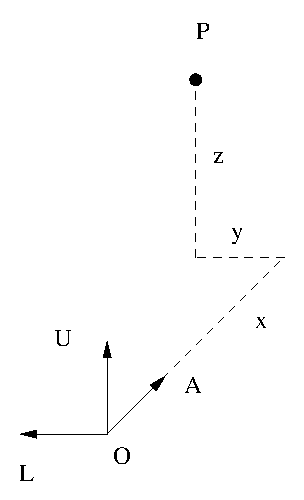
\includegraphics[height=2in]{../images/projector.eps}
%
& \hspace{2cm} &
%
%\begin{figure}[h]
  \psfrag{P}{$P(a,b,c)$}
  \psfrag{O}{$O(0,0,0)$}  
  \psfrag{x}{$a$} 
  \psfrag{y}{$b$} 
  \psfrag{z}{$c$}     
  \psfrag{A}{$Ox$}
  \psfrag{L}{$Oy$}
  \psfrag{U}{$Oz$}  
  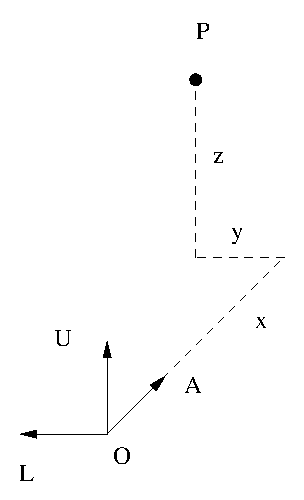
\includegraphics[height=2in]{../images/projector.eps}
%
\end{tabular}
  \end{table}
%
\end{frame}

\begin{frame}[label=current]
 \frametitle{Euclidean Distance in Coordinates}

   Points $A(x_A,y_A,z_A)$ and $B(x_B,y_B,z_B)$:
   %
\begin{figure}[h]
  \psfrag{O}{$O$}
  \psfrag{A}{$A$} 
  \psfrag{B}{$B(x_B, y_B, z_B)$}  
  \psfrag{C}{$C(x_B, y_B, z_A)$}    
  \psfrag{x}{$y$} 
  \psfrag{y}{$x$} 
  \psfrag{z}{$z$}     
  \psfrag{dx}{$y_B - y_A$}
  \psfrag{dy}{$x_B - x_A$}
  \psfrag{dz}{$z_B - z_A$}  
  \includegraphics[height=2in]{../images/euclidean_distance.eps}
  %\caption{Euclidean distance}
  %\label{fig:euclidean_distance}
\end{figure}
%
$$d(A,B) = |AB| = \sqrt{(x_B-x_A)^2+(y_B-y_A)^2+(z_B-z_A)^2}$$
%
Example: $P(3,1,2)$ and $Q(1,2,3)$:\pause
%
$$D(P,Q) = \sqrt{(1-3)^2+(2-1)^2+(3-2)^2} = \sqrt{6}\; .$$

\end{frame}

\begin{frame}
 \frametitle{Change of Coordinates}

  Change in original position and orientation $\to$ new coordinates

\pause

Example:
  \begin{itemize}
   \item Move ahead 1m;
   \item Turn a quarter of a circle to the right.
  \end{itemize}
  
%
\begin{table}[h]
\begin{tabular}{lcr}
  \psfrag{P}{$P(3,1,2)$}
  \psfrag{O}{$O(0,0,0)$}  
  \psfrag{x}{$x=3$} 
  \psfrag{y}{$y=1$} 
  \psfrag{z}{$z=2$}     
  \psfrag{A}{$Ox$}
  \psfrag{L}{$Oy$}
  \psfrag{U}{$Oz$}  
  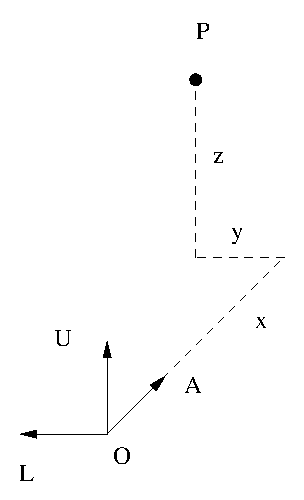
\includegraphics[height=2in]{../images/projector.eps}
%
& \hspace{2cm} &
%
\psfrag{P}{$P$}
  \psfrag{Op}{$O'$} 
  \psfrag{O}{$O$}  
  \psfrag{L}{$L$}
  \psfrag{U}{$U$}   
  \psfrag{xp}{$x'=-1$} 
  \psfrag{yp}{$y'=2$} 
  \psfrag{zp}{$z'=2$}     
  \psfrag{Ap}{$A'$}
  \psfrag{Lp}{$L'$}
  \psfrag{Up}{$U'$}  
  \includegraphics[height=2in]{../images/new_frame.eps}
%
\end{tabular}
  \end{table}
%  
%
\pause  
New coordinates of projector: $P \to (x',y',z') = (-1,2,2)$
\end{frame}

\begin{frame}
\frametitle{General formula for this change of coordinates}
%
\begin{table}[h]
\begin{tabular}{lcr}
  \psfrag{P}{$P(x,y,z)$}
  \psfrag{O}{$O(0,0,0)$}  
  \psfrag{x}{$x$} 
  \psfrag{y}{$y$} 
  \psfrag{z}{$z$}     
  \psfrag{A}{$Ox$}
  \psfrag{L}{$Oy$}
  \psfrag{U}{$Oz$}  
  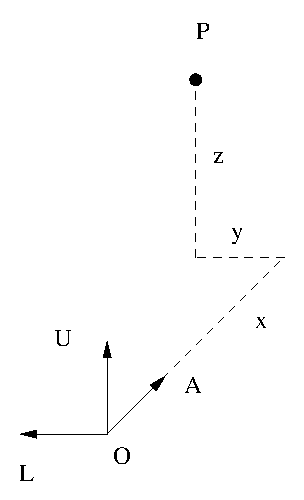
\includegraphics[height=2in]{../images/projector.eps}
%
& \hspace{2cm} &
%
\psfrag{P}{$P(x', y', z')$}
  \psfrag{Op}{$O'$} 
  \psfrag{O}{$O$}  
  \psfrag{L}{$L$}
  \psfrag{U}{$U$}   
  \psfrag{xp}{$x'=-y$} 
  \psfrag{yp}{$y'=x-1$} 
  \psfrag{zp}{$z'=z$}     
  \psfrag{Ap}{$A'$}
  \psfrag{Lp}{$L'$}
  \psfrag{Up}{$U'$}  
  \includegraphics[height=2in]{../images/new_frame.eps}
%
\end{tabular}
  \end{table}
%  

\begin{eqnarray*}
 x' = & -y \\
 y' = & x-1 \\
 z' = & z
\end{eqnarray*}
%
Example $Q(x=1,y=2,z=3) \leftrightarrow Q(x'=-2, y'=0,z'=3)$

\end{frame}



\begin{frame}
 \frametitle{Fundamental Philosophy}
  $P(3,1,2)$ and $Q(1,2,3)$ in $(x,y,z)-$coordinates

  $P(-1,2,2)$ and $Q(-2,0,3)$ in $(x',y'z')-$coordinates

  Distance in new coordinates:
 \pause
%
$$d_{x',y',z'}(P,Q) = \sqrt{(-2+1)^2+(0-2)^2+(3-2)^2} = \sqrt{6} = d_{x,y,z}(P,Q)$$

Fundamental Philosophy:\pause
\begin{itemize}
 \item Space doesn't come with coordinates
  \item Natural concepts (such of distance) are independent of coordinates
  \item If a natural concept is defined using coordinates, \\
          the result does not depend on the chosen coordinate system.
\end{itemize}


\end{frame}

\begin{frame}
  \frametitle{Sets in Space}

  $X$ subset of a set $Y$:

  $$X = \{ A \text{ in } Y | A \text{ has property } \mathcal{P} \} \subset Y$$

\pause
Examples  (Fixed point $Q$, fixed $r>0$):

$$X = \{ A \text{ in Space } | d(A,Q) = r \} = S_r(Q)\; ,$$
\pause Sphere of radius $r$ centered at $Q$.\pause

$$B_r(Q) = \{ A \text{ in Space } | d(A,Q) <r \} \; ,$$
\pause  Open ball of radius $r$ centered at $Q$. \pause

$$\overline{B}_r(Q) = \{ A \text{ in Space } | d(A,Q) \leqslant r\} \; ,$$
\pause  Closed ball of radius $r$ centered at $Q$.

\end{frame}

\begin{frame}
 \frametitle{Equation(s) of Subsets}

  $$X = \{ (x,y,z) | x,y,z \text{ satisfy certain relation(s) } \} \; .$$

\pause
Examples:

$\{(x,y,z) | x^2+y^2+z^2 = 1\}$:

\pause
sphere of radius $r=1$ centered at the origin $(0,0,0)$

Also refered to as: sphere $x^2+y^2+z^2 = 1$

\pause
\medskip

$\{ (x,y,z) | x=0 \}$: coordinate Left-Up plane

\pause
\medskip

$\{ (x,y,z) | x=0 \text{ and } y=0 \}$:

intersection of coordinate planes $\rightarrow$ coordinate axis

\pause
\medskip

Can be given by only one equation:

$x^2+y^2 = 0$ $\rightarrow$ $x=0$,$y=0$, and $z$ arbitrary $\rightarrow$

vertical axis above $(0,0)$ in $(x,y)-$plane

\pause
\medskip

Important: Equations in Plane vs. Space.

\end{frame}

\begin{frame}
 \frametitle{Recognizing Spheres from Equations}

  $Q(x_0,y_0,z_0)$, $r>0$, $A(x,y,z)$. Remark: $d(A,Q) = r \longleftrightarrow d^2(A,Q) = r^2$

$$S_r(Q): \quad (x-x_0)^2+(y-y_0)^2+(z-z_0)^2 = r^2$$

\pause
Example:
$$(x-2)^2+(y-0)^2+(z+1)^2=3^2$$
%
$$x^2+y^2+z^2 -4x + 2z -4=0$$

\pause
\begin{itemize}
 \item no mixed terms $xy$, $xz$, or $yz$;
 \item quadratic terms $x^2$, $y^2$, and $z^2$ with the same coefficient.
\end{itemize}

\pause
Examples:
$$x^2+y^2+z^2-4x+2y=0$$
%
\pause
Complete the square:
%
$$(x-2)^2 + (y+1)^2 +z^2 = 5$$
%
Sphere of radius $\sqrt{5}$ centered at $(2,-1,0)$.

\pause
How about $x^2+y^2+z^2 - 4x+2y = -6$? \pause Passes both tests, but ...
%
$$(x-2)^2 + (y+1)^2 +z^2 = -1$$
%
is impossible! No such points, set is empty.

\end{frame}

\begin{frame}
 \frametitle{Polar Coordinates}
%
\begin{figure}[h]
  \psfrag{Q}{$Q$}
  \psfrag{O}{$O$}
  \psfrag{Qx}{$Q_{x}$}
  \psfrag{Qy}{$Q_{y}$}
  \psfrag{x}{${x}$}
  \psfrag{y}{${y}$}
  \psfrag{xq}{$x_Q$}
  \psfrag{yq}{$y_Q$} 
  \psfrag{th}{$\theta_Q$}
  \psfrag{r}{$r_Q$}  
  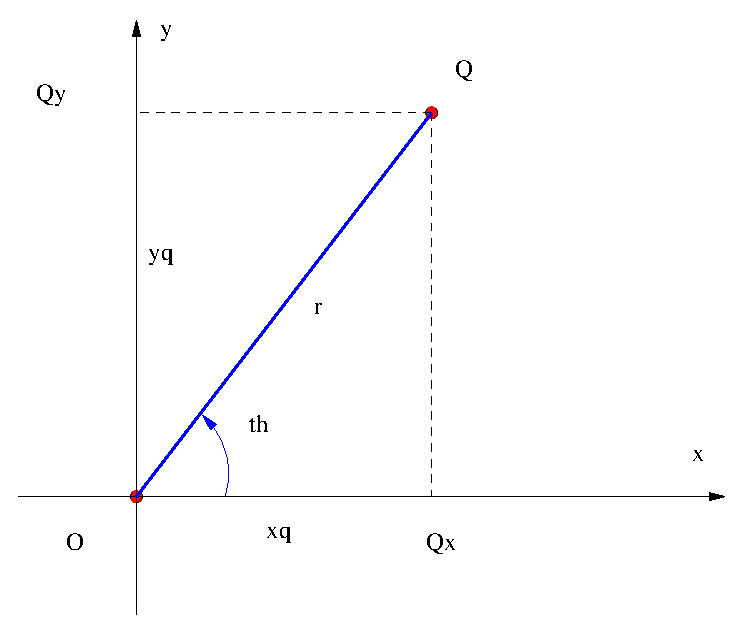
\includegraphics[height=1.5in]{../images/polar_coordinates.eps}
  %\caption{Polar coordinates}
\end{figure}
%
\begin{itemize}
 \item $r$: distance from $O$ to $Q$;

  \item $\theta$: angle from $Ox$ to $OQ$\\
    measured counterclockwise
\end{itemize}

\pause
Range of coordinates:
\begin{itemize}
 \item $r$: \pause $[0, \infty)$
  \item $\theta$:\pause $[0, 2\pi)$, for example
\end{itemize}

\end{frame}


\begin{frame}
 \frametitle{Transition Polar - Rectangular}
%
\begin{figure}[h]
  \psfrag{Q}{$Q$}
  \psfrag{O}{$O$}
  \psfrag{Qx}{$Q_{x}$}
  \psfrag{Qy}{$Q_{y}$}
  \psfrag{x}{${x}$}
  \psfrag{y}{${y}$}
  \psfrag{xq}{$x_Q$}
  \psfrag{yq}{$y_Q$} 
  \psfrag{th}{$\theta_Q$}
  \psfrag{r}{$r_Q$}  
  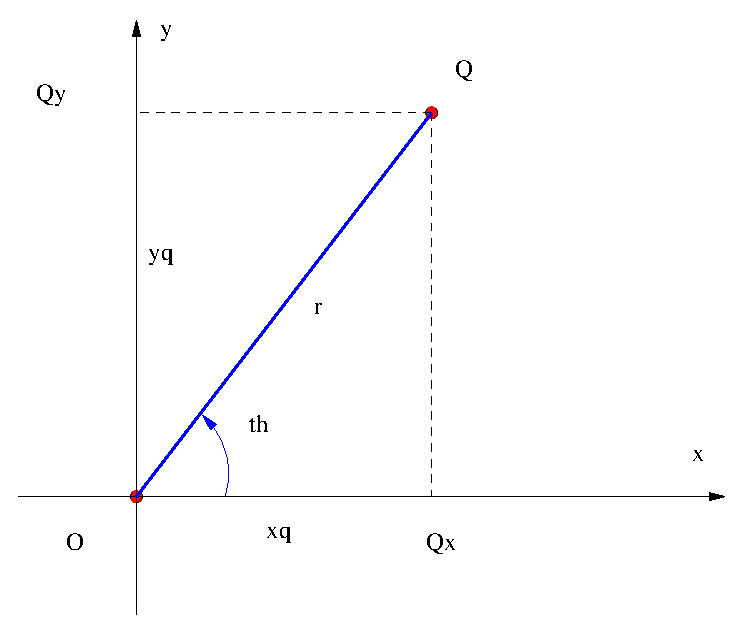
\includegraphics[height=1.5in]{../images/polar_coordinates.eps}
  %\caption{Polar coordinates}
\end{figure}
%
Polar to rectangular:\pause
$$ x = r \cos\theta \quad , \quad y = r\sin\theta$$

Rectangular to polar:\pause
$$ r = \sqrt{x^2+y^2}$$
$$\cos\theta = \frac{x}{r} \quad , \quad \sin\theta = \frac{y}{r}\; .$$

\end{frame}

\begin{frame}
 \frametitle{Cylindrical coordinates}
%
\begin{figure}[h]
  \psfrag{P}{$P$}
  \psfrag{O}{$O$}  
  \psfrag{xp}{$x_P$} 
  \psfrag{yp}{$y_P$} 
  \psfrag{zp}{$z_P$}     
  \psfrag{rp}{$r_P$}
  \psfrag{thp}{$\theta_P$}
  \includegraphics[height=2in]{../images/cylindrical_coordinates.eps}
  %\caption{Cylindrical coordinates}
  %\label{fig:cylindrical-coordinates}
\end{figure}
%
$$P(x,y,z) \Longleftrightarrow P(r, \theta, z)$$

\begin{itemize}
    \item Polar in $Oxy$ -- $(r, \theta)$;
    \item Rectangular in $Orz$ -- $(r, z)$.
\end{itemize}

\end{frame}

\begin{frame}
%
\begin{figure}[h]
  \psfrag{P}{$P$}
  \psfrag{O}{$O$}  
  \psfrag{xp}{$x_P$} 
  \psfrag{yp}{$y_P$} 
  \psfrag{zp}{$z_P$}     
  \psfrag{rp}{$r_P$}
  \psfrag{thp}{$\theta_P$}
  \includegraphics[height=2in]{../images/cylindrical_coordinates.eps}
  %\caption{Cylindrical coordinates}
  %\label{fig:cylindrical-coordinates}
\end{figure}
%
Cylindrical to rectangular:\pause
$$x=r\cos\theta \quad , \quad y = r\sin\theta \quad , \quad z_{r} = z_{c}$$

Rectangular to cylindrical:\pause
$$r= \sqrt{x^2+y^2} \quad , \quad z_{c}=z_{r}$$
$$\cos\theta = \frac{x}{r} \quad , \quad \sin\theta = \frac{y}{r}\; .$$
\end{frame}

\begin{frame}
 \frametitle{Constant Coordinate Sets}
 \begin{table}[h]
\begin{tabular}[t]{lr}
  \psfrag{P}{$P$}
  \psfrag{O}{$O$}  
  \psfrag{xp}{$x_P$} 
  \psfrag{yp}{$y_P$} 
  \psfrag{zp}{$z_P$}     
  \psfrag{rp}{$r_P$}
  \psfrag{thp}{$\theta_P$}
  \includegraphics[height=2in]{../images/cylindrical_coordinates.eps}
&
{\parbox{0.5\textwidth}{
Surfaces:
\begin{itemize}
  \item $r$ constant \pause$\to$ vertical cylinder;
  \item $\theta$ constant \pause$\to$ vertical half plane;
  \item $z$ constant \pause$\to$ horizontal plane.\pause
\end{itemize}
%
Curves:
\begin{itemize}
 \item $\theta, z$ constant \pause$\to$ horizontal ray;
\item $r, z$ constant \pause$\to$ horizontal circle;
\item $r, \theta$ constant \pause$\to$ vertical line.
\end{itemize}
}}
%
\end{tabular}
\end{table}

\end{frame}

\begin{frame}
 \frametitle{Spherical Coordinates}
%
\begin{table}[h]
\begin{tabular}[t]{lr}
  %  
  %
  \psfrag{P}{$P$}
  \psfrag{O}{$O$}  
  \psfrag{xp}{$x_P$} 
  \psfrag{yp}{$y_P$} 
  \psfrag{zp}{$z_P$}     
  \psfrag{rho}{$\rho_P$}
  \psfrag{thp}{$\theta_P$}
  \psfrag{phi}{$\phi_P$}
  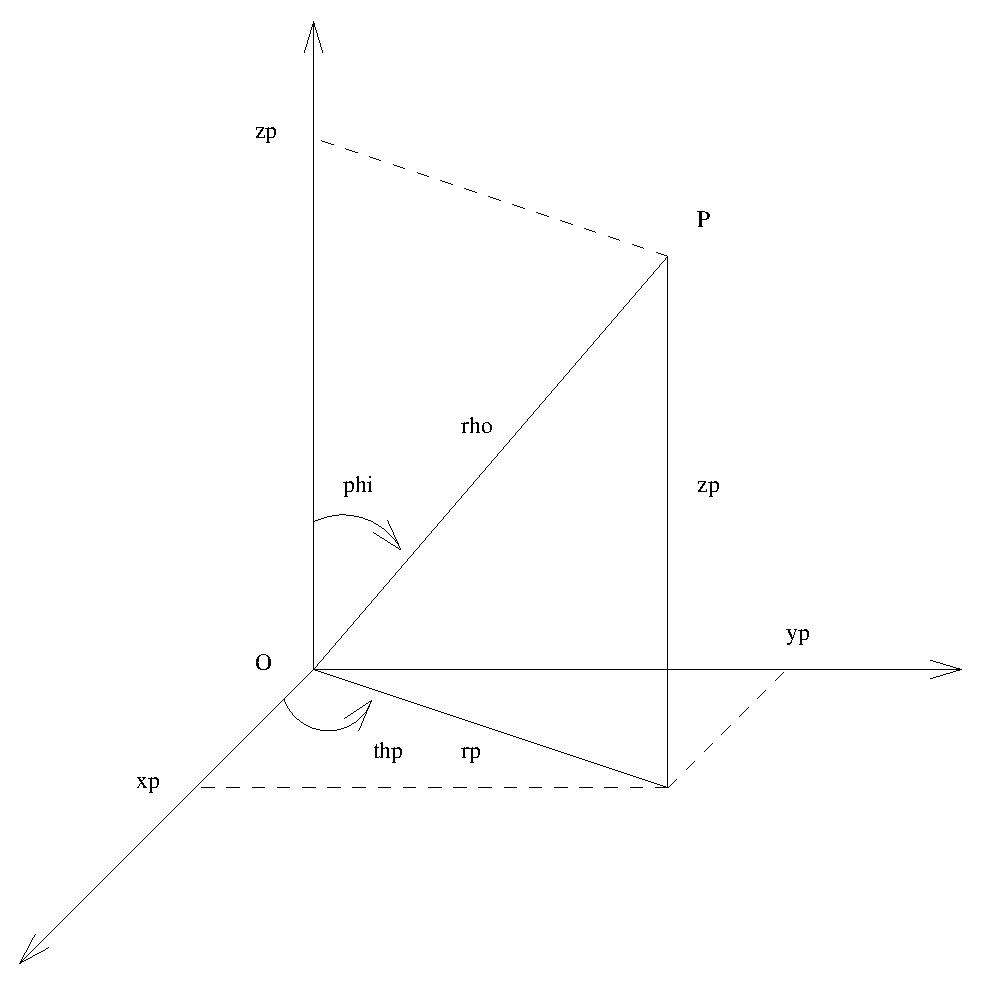
\includegraphics[height=2in]{../images/ok-cylindrical-spherical.eps}
%
&
{\parbox{0.4\textwidth}{
Coordinates:
	\begin{itemize}
 	\item $\rho$: distance $|OP|$;
	\item $\phi$: angle $Oz$ to $OP$;
	\item $\theta$: angle $Ox$ to $OP_{xy}$.
	\end{itemize} 

Combination:
\begin{itemize}
    \item Polar in $Oxy$ -- $(r, \theta)$;
    \item Polar in $Ozr$ -- $(\rho, \phi)$.
\end{itemize}

Range of coordinates:
\begin{itemize}
 \item $\rho$:  $[0,\infty)$;
  \item $\phi$:  $[0, \pi]$;
  \item $\theta$:  $[0,2\pi)$.
\end{itemize}
}}
\end{tabular}
  \end{table}

\end{frame}

\begin{frame}
 \frametitle{Transition Spherical - Rectangular}

\pause
Spherical to rectangular:\pause
\begin{align*}
 x & = r\cos\theta = \rho\sin\phi \cos\theta \\
  y & = r\sin\theta = \rho\sin\phi \sin\theta \\
  z & = \rho\cos\phi
\end{align*}

\pause
Rectangular to spherical:\pause
$$\rho = \sqrt{x^2+y^2+z^2} \quad , \quad r = \sqrt{x^2+y^2}$$
$$\cos\phi = \frac{z}{\rho} \quad , \quad \sin\phi = \frac{r}{\rho}$$
$$\cos\theta = \frac{x}{r} \quad , \quad \sin\theta = \frac{y}{r}$$

\end{frame}

\begin{comment}
\begin{frame}
 \frametitle{Curvilinear boxes}
 
 Polar ``wedge'':
 %
$$C  = \{ P(r,\theta) \; | \;r_0 \leqslant
r \leqslant r_0+\Delta r,  \theta_0 \leqslant \theta
\leqslant \theta_0+\Delta \theta\} \; .$$
%
Shape? \pause Area = ...?
\pause

\bigskip

Cylindrical ``box'':
%
$$X = \{ P(r,\theta, z) \; | \; 0 \leqslant r \leqslant r_0\, ,
0 \leqslant \theta \leqslant \theta_0\, ,
0 \leqslant z \leqslant z_0\}$$

\pause
Shape ? \pause Volume = ...?

\bigskip

\pause
Spherical ``box'':
%
$$Y = \{ P(\rho, \phi, \theta) \; | \; 0 \leqslant \rho \leqslant \rho_0\, ,
0 \leqslant \phi \leqslant \phi_0\, ,
0 \leqslant \theta \leqslant \theta_0\}$$

\pause
Shape? \pause Volume = ...?

\end{frame}
\end{comment}
